\begin{enumerate}[label=\thesection.\arabic*.,ref=\thesection.\theenumi]
\numberwithin{equation}{enumi}

\item Loop Tranfer function of a feedback system is 
\begin{align}
G(s)H(s) = \frac{s+3}{s^2(s-3)}
\label{eq:es17btech11009_system}
\end{align}
Take the Nyquist contour in the clockwise direction.
\\
Then the Nyquist plot of G(s)H(s) encircles -1 + j0
\\
(A) Once in clockwise direction
\\
(B) Twice in clockwise direction
\\
(C) Once in anticlockwise direction
\\
(D) Twice in clockwise direction
\\
\\
\solution Substituting $s = \j\omega$ in \eqref{eq:es17btech11009_system},
\begin{align}
G\brak{\j\omega}H\brak{\j\omega}&=\frac{j\omega+3}{(j\omega)^2\brak{j\omega- 3}}
\\
G\brak{\j\omega}H\brak{\j\omega}&=\frac{j\omega+3}{\omega^2\brak{3 - j\omega}}
\end{align}

\begin{align}
\abs{G\brak{\j\omega}H\brak{\j\omega}}&=\frac{\brak{\sqrt{\omega^2+9}}}{(\omega)^2\brak{\sqrt{\omega^2+9}}}
\\
\abs{G\brak{\j\omega}H\brak{\j\omega}}&=\dfrac{1}{(\omega)^2}
\label{eq:es17btech11009_mag}
\end{align}

\begin{align}
\angle{G\brak{\j\omega}H\brak{\j\omega}}&=\tan^{-1}\brak{\frac{\omega}{3}} - (\pi/2 + \pi/2 -  \tan^{-1}\brak{\frac{\omega}{3}} )
\\
\angle{G\brak{\j\omega}H\brak{\j\omega}}&= 2\tan^{-1}\brak{\frac{\omega}{3}}
\label{eq:es17btech11009_phase}
\end{align}

\item Find $G(j\omega)H(j\omega)$ for the Nyquist plotting

\solution From \eqref{eq:es17btech11009_mag} and \eqref{eq:es17btech11009_phase} 

\begin{align}
G\brak{\j\omega}H\brak{\j\omega}&= \dfrac{1}{(\omega)^2}\angle2\tan^{-1}\brak{\frac{\omega}{3}}
\end{align}

\item Nyquist plot and verify your result

\solution
 For the Nyquist plot, 
\\
We need to draw the polar plot by varying $\omega$  \ from \ 0 \ to  \ \infty

\begin{align}
 \lim_{\omega\to \infty}{G\brak{\j\omega}H\brak{\j\omega}} &= 0\angle{180}
\end{align}
\begin{align}
\lim_{\omega\to 0}{G\brak{\j\omega}H\brak{\j\omega}} &= \infty\angle{0}
\end{align}
The Nyquist plot is as shown

\begin{figure}[!h]
\centering
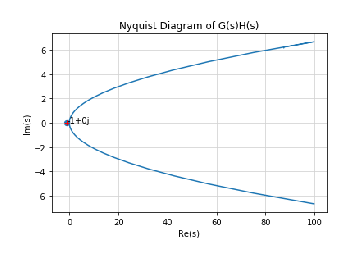
\includegraphics[width=\columnwidth]{./figs/es17btech11009.eps}
\caption{}
\label{fig:es17btech11009_1}
\end{figure}

Since there are two poles on the origin we get 2 infinite radius semicircles which start where the mirror image ends and terminate where the actual plot started in clockwise direction.
\begin{lstlisting}
codes/es17btech11009.py
\end{lstlisting}

 Above code gives us the Nyquist plot


The Nyquist plot of G(s)H(s) encircles -1 + j0 once in clockwise direction


\end{enumerate}
